\documentclass[a4paper,10pt]{article}
\usepackage[utf8]{inputenc}
\usepackage[margin=3cm]{geometry}
\usepackage{amsmath}
\usepackage{amssymb}
\usepackage{amsthm}
\usepackage{fancyhdr}
\usepackage{seminar}
\usepackage{graphicx}
\usepackage{subfigure}
\usepackage{float}
\usepackage{hyperref}
\usepackage{mathtools}

\pagestyle{fancy}

\graphicspath{ {../Presentation/}}

%You can add theorem-like environments (e.g. remark, definition, ...) if you want
\newtheorem{theorem}{Theorem}

\title{Generalization Ideas in Deep Learning} % Replace with your title
\author{Marcel Bruckner} % Replace with your name
\institute{\textit{Seminar: Optimization and Generalization in Deep Learning}}

\makeatletter
\let\runauthor\@author
\let\runtitle\@title
\makeatother
\lhead{\runauthor}
\rhead{\runtitle}

\newcommand{\signed}[1]{%
	{\unskip\nobreak\hfil\penalty50
		\hskip2em\hbox{}\nobreak\hfil#1
		\parfillskip=0pt \finalhyphendemerits=0 \par}}
\newcommand\inlineeqno{\signed{\stepcounter{equation}\ (\theequation)}}
\newcommand{\fref}[1]{(Fig:~\ref{#1})}
\newcommand{\freff}[1]{Figure~\ref{#1}}
\newcommand{\sref}[1]{Section~\ref{#1}}
\newcommand{\ns}{Neyshabur~et~al.~\cite{neyshabur2017exploring}}

\begin{document}

\maketitle

\begin{abstract}
Trying to understand the generalization abilities of deep neural networks several capacity measures are experimentally explored. Following the thoughts of \ns{} different norm-based capacity measures on the network weights and sharpness as the robustness to perturbations on the parameter space are investigated. The measures are used in different experiments and the results are plotted against each other.
\end{abstract}

\section{Introduction}
In recent years we have seen the huge empirical success of deep neural networks. Even though they solve complex, highly non-convex optimization problems simple stochastic gradient descent methods achieve good generalization behavior in practice. We see that even in the highly over parameterized regime in which deep neural networks are located many of the local minima provide good generalization on unseen data. Nonetheless, it remains mostly unclear why they exhibit the desired generalization behavior.\\
%
\ns{} provided us with a methodology to investigate into measures of the generalization ability. Using this framework we tried to reproduce their results and to understand how different measures on the parameter space can explain certain empirical phenomena that are directly connected to generalization abilities of deep neural networks.
%
%!TEX root=./report.tex

\section{Capacity control}
\ns{} examined complexity measures that have recently been suggested, or could be considered, in explaining generalization in deep learning. They evaluated the measures based on their ability to theoretically guarantee generalization, and their empirical ability to explain the phenomena discussed in \sref{sec:empricial-study}. 
%
\subsection{Norm-based capacity control}
For deep neural networks a multitude of norm-based regularization techniques on the network weights have been established. Different approaches, e.g. the $l1/l2$ norms, their respective path norms \cite{DBLP:journals/corr/NeyshaburSS15} or the spectral and nuclear norm are used to control the capacity of networks independent of the number of parameters.
%
\paragraph{Margin}
To meaningful compare norms of deep neural networks we have to explicitly take into account the scaling of the outputs of the network. As we drive the training error to zero we have to push the cross entropy loss to zero and thus the outputs of the network must go to infinity. This means that minimizing the cross entropy loss will drive the norms towards infinity. \\
In practice, we will stop the training after some finite time and the norm of the network will be large but also finite. The resulting norm value will mostly be an indicator on how far the training has progressed.\\
To overcome this scaling issues \cite{neyshabur2017exploring} suggested using the margin over the whole training set, where the margin for a single data point is the difference between the score of the correct label and the maximum score of other labels $f_w(x)[y_{true}] - max_{x \neq y_{true}}f_w(x)[y]$. As taking the minimum margin over the whole training set is really sensitive to outliers \cite{neyshabur2017exploring} defined the $\gamma_{margin}$ as the lowest value of $\gamma$ such that $\lceil\epsilon m\rceil$ data points have margin lower than $\gamma$, where m is the size of the training set and $\epsilon > 0$ is small.
%
\paragraph{Norms}
The measures investigated by \cite{neyshabur2017exploring} and the corresponding capacity bounds are as follows:
%
\begin{itemize}
	\item $l2$ norm with capacity proportional to $\frac{1}{\gamma_{margin}^2} \prod_{i=1}^{d} 4 \left\| W_i  \right\|_F^2$ \inlineeqno
	\item $l1$-path norm with capacity proportional to $\frac{1}{\gamma_{margin}^2} \left| \sum_{j \in \prod_{k=0}^d[h_k]}^{} \left| \prod_{i=1}^{d} 2 W_i [j_i, j_{i-1}] \right|\right|^2$ \inlineeqno
	\item $l2$-path norm with capacity proportional to $\frac{1}{\gamma_{margin}^2} \sum_{j \in \prod_{k=0}^d[h_k]}^{} \prod_{i=1}^{d} 4 h_i W_i^2 [j_i, j_{i-1}]$ \inlineeqno
	\item spectral norm with capacity proportional to $\frac{1}{\gamma_{margin}^2} \prod_{i=1}^{d} h_i \left\| W_i  \right\|_2^2$ \inlineeqno
\end{itemize}
where $\prod_{i=1}^{d}\dots$ is the product over all network layers, $h_i$ is the number of hidden units in layer $i$ and $\prod_{k=0}^d[h_k]\dots$ is the Cartesian product over sets $[h_k]$ and displays the enumeration of all paths through the network from input to output nodes.
%
\subsection{Sharpness}
Keshkar er al. \cite{DBLP:journals/corr/KeskarMNST16} recently suggested sharpness as a generalization measure that corresponds to robustness to adversarial perturbations on the parameter space:
%
\begin{equation}
\zeta _\alpha (w) = \frac{\max_{\left| \nu_i \right| \le \alpha(\left| w_i  \right| + 1) }\hat{L}(f_{w + \nu}) - \hat{L}(f_w)}{1 + \hat{L}(f_w)} \cong \max_{\left| \nu_i \right| \le \alpha(\left| w_i  \right| + 1) }\hat{L}(f_{w + \nu}) - \hat{L}(f_w)
\end{equation}
% 
where $\hat{L}(f_{w})$ is the empirical loss over the whole training set and generally very small, so we can drop it from the denominator.


%!TEX root=./report.tex
\section{Empirical study}
In this section we discuss the experimental results using the proposed measures and their implications on different phenomena seen in practice regarding the generalization behavior.
%
\subsection{Difference between true and random labeled data}
\begin{figure}
	\centering
	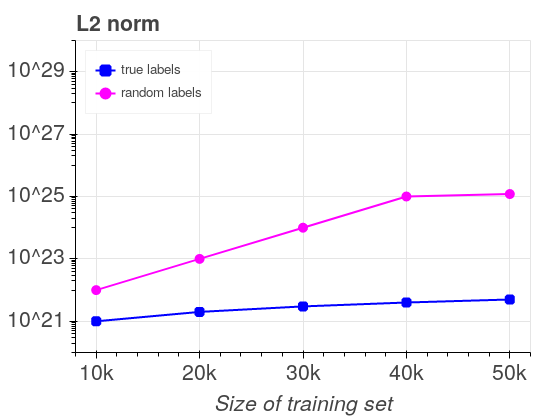
\includegraphics[width=0.24\linewidth]{vgg16/bokeh_plot.png}
	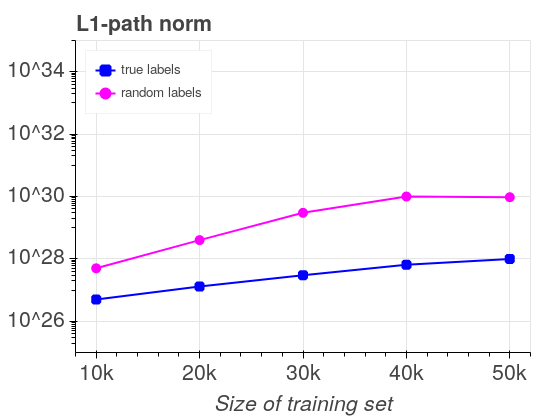
\includegraphics[width=0.24\linewidth]{vgg16/bokeh_plot(1).png}
	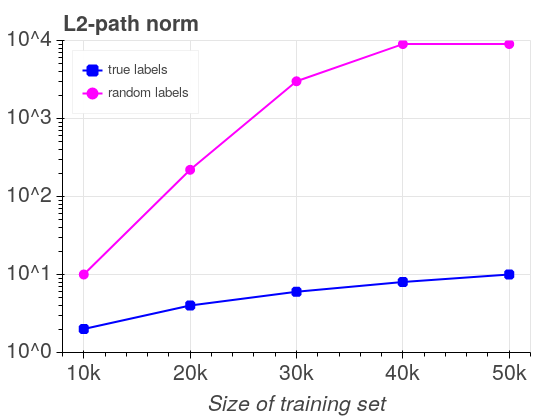
\includegraphics[width=0.24\linewidth]{vgg16/bokeh_plot(2).png}\\
	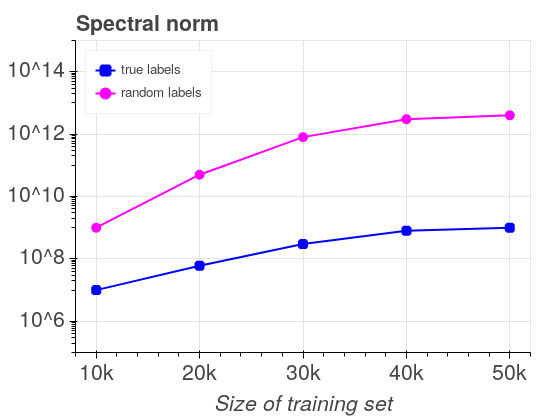
\includegraphics[width=0.24\linewidth]{vgg16/bokeh_plot(3).png}
	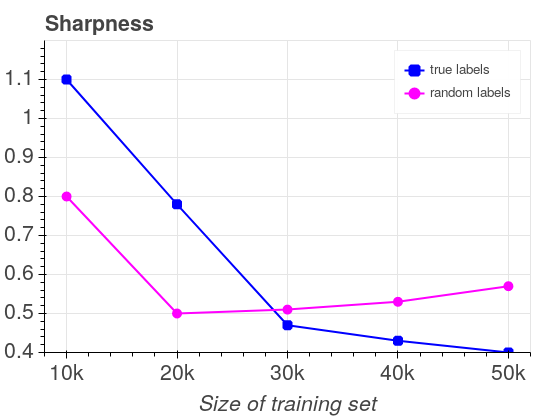
\includegraphics[width=0.24\linewidth]{vgg16/bokeh_plot(4).png}
	\caption{The proposed capacity measures calculated on the VGG model \cite{simonyan2014deep} after training on random (magenta) and true (blue) labeled subsets of CIFAR-10. We see only a small increase of the measures on true labels but a huge increase using random labels and the measures on random labels to be bigger for every subset. Reproduced from \cite{neyshabur2017exploring}.}	
	\label{fig:norms-paper}
\end{figure}
It is possible to obtain zero training error on random labels using the same architecture for which training with real labels leads to good generalization. We would expect the networks learned using real labels (and which generalizes well) to have much lower complexity, under the suggested measure, than those learned using random labels (and which obviously do not generalize well). \cite{neyshabur2017exploring} \par
%
\freff{fig:norms-paper} shows the results of \cite{neyshabur2017exploring}. We see that training the network on true labels (blue) only results in small increases of the norm-based capacity measures in comparison to the increases when training on random labels (magenta). As the network learns the true functional dependence between the input and output using true labels it only requires small increases in complexity as the subset size increases, whereas it requires more capacity for every newly seen data point when using random labels as it needs to memorize the data point.\\
We also see that the norm-based capacity measures are all bigger for random labeled data as the network has to memorize the data whereas the dependence between the input and output can be learned with lower capacity on true labeled data. \par
%
Looking at the sharpness as a capacity measure in \freff{fig:norms-paper} we do not see a direct correlation between its value and the capacity of the network. We expect the model to become less sharp when increasing the network size which can be seen looking at the true labeled data points (blue) but clearly gets violated by the random labeled data points (magenta). Furthermore, we see a lower sharpness for random labels for the two smallest subset sizes which contradicts the intuition that the sharpness should be always lower for true labels. 
%
\subsubsection{Problems reproducing results}
\label{sec:problems-subset-sizes}
\begin{figure}
	\centering
	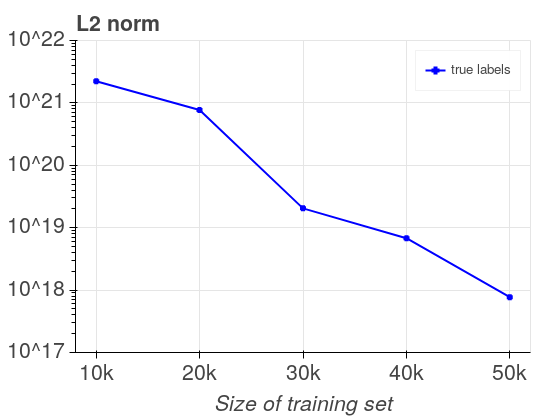
\includegraphics[width=0.24\linewidth]{vgg16/l2_own.png}
	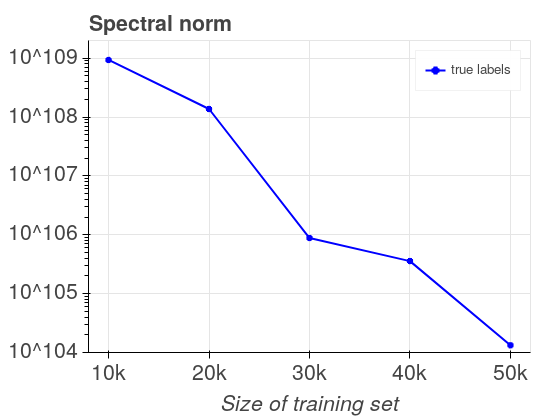
\includegraphics[width=0.24\linewidth]{vgg16/spectral_own.png}
	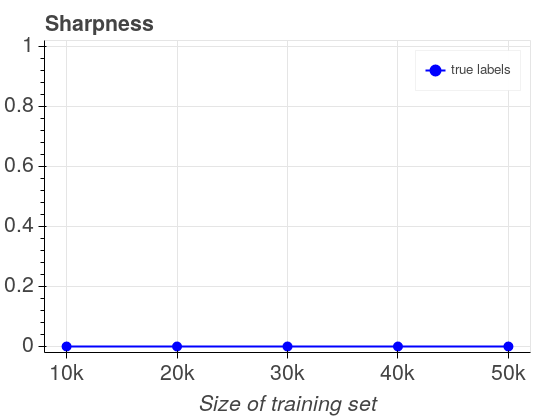
\includegraphics[width=0.24\linewidth]{vgg16/sharpness_own.png}
	\caption{Our own results for the $l2$ and spectral norm as well as the sharpness calculated on the VGG-16 model after training on subsets of CIFAR-10. The results show no reproducibility of the results presented by \cite{neyshabur2017exploring}.}	
	\label{fig:norms-own}
\end{figure}
Following the vague instructions of \cite{neyshabur2017exploring} the VGG-16 network with batch normalization \fref{fig:cifar-vgg} is trained on different subsets of the CIFAR-10 \fref{fig:cifar-vgg} data set. For every subset a copy with the labels replaced by random labels has been created and the model is trained on both the true and random labeled subset. \\
%
The huge scope for interpretation of the approach used in \cite{neyshabur2017exploring} caused the non reproducibility of the results which are shown in \freff{fig:norms-own}. The problems we face are:
%
\paragraph{Reproduction of network training}
\label{sec:problems-reproduction-training}
\ns{} only stated that their results were produced using VGG. As VGG is a class of CNN architectures with varying depths and optional batch normalization we performed a grid search over the implementations. Considering the capacity vs. training time trade-of we achieved the best results using VGG-16 with batch normalization.\\
Furthermore, \cite{neyshabur2017exploring} didn't provide information on the used solving strategy. Therefore, we tried simple stochastic gradient descent and Adam but stuck with the later as of the faster convergence.
%
\paragraph{Calculation of norms}
\label{sec:problems-calculation-norms}
The calculation of path norms is trivial for the fully connected case but not for convolutional layers. As we need to enumerate every path through the network we need a way to associate the layer neurons of succeeding layers when applying a convolution. In the short time of this paper we couldn't come up with a feasible implementation which made it impossible to reproduce the path norms.
%
\paragraph{Training on random labeled data}
Following the missing details of the network implementation and solving strategy a training on random labeled data was not possible. The network didn't overcome a $1/10$ test accuracy on random labels which represents a random choice of the result by the network out of the $10$ classes in the CIFAR-10 data set.

\paragraph{Training time}
\label{sec:problems-training-time}
The short scope of the seminar enclosing this paper combined with training times ranging from roughly five hours on the smallest subset ranging up to over one day for the biggest one resulted in only small search intervals for the grid search used on the hyper parameters as well for the algorithmic and architectural choices.
%
\paragraph{Sharpness}
\label{sec:problems-sharpness}
Sharpness as the maximum over the adversarial perturbations is a maximization problem where the difference between the loss of the network with the added perturbation and the original network gets maximized. This maximization problem is constrained on the values of the perturbations and thus requires a constrained optimization strategy. We couldn't come up with such a strategy in the seminars time and thus tried a random search strategy. Due to the high duration of forward passes over the whole training set this random search didn't provide results in a feasible amount of time.
%
%
%%%%%%%%%%%%%%%%%%%%%%%%%%%%%%%%%%%%%%%%%%%%%%%%%%%%%%%%%%%%%%%%%%%%%%%%%%%%%%%%%%%%%%%%%%%%%%%%%%%%%%%%%%%%%%%%%%%%%%%%%%%%%%%%%%
%
%
%
\subsection{Difference between local minima}
When training the same architecture, with the same training set, using two different optimization methods (or different algorithmic or parameter choices), one method results in better generalization even though both lead to zero training error. We would
expect to see a correlation between the complexity measure and generalization ability among zero-training error models. \cite{neyshabur2017exploring} \par
%
To drive the network towards different parameter choices \cite{neyshabur2017exploring} proposed to train the VGG network \cite{simonyan2014deep}\fref{fig:cifar-vgg} on a subset of 10000 true labeled data points of the CIFAR-10 \fref{fig:cifar-vgg} and to add confusion sets with varying sizes. A confusion set is a subset of the same data set where the labels are replaced with random labels. When optimizing the network over the union of the true and random labeled sets the resulting optimum has to be optimal for both of the sets.\\
%
We expect to see an increase of the test error with increasing confusion set size as the network not only has to learn the functional dependence between the input and output data but also has to memorize an increasing number of random labeled data points.
This memorization prevents the network from generalizing well and can be seen in \freff{fig:confusion-paper}.\\
%
Following the increase in test error and the resulting worse generalization behavior we expect the capacity measure to increase with the test error. In \freff{fig:confusion-paper} we see this behavior for all the norm-based capacity measures which hints towards them being a valid measure for generalization behavior. But again we see the sharpness to have no direct correlation to the test error which hints that it cannot predict generalization.
%
\begin{figure}
	\centering
	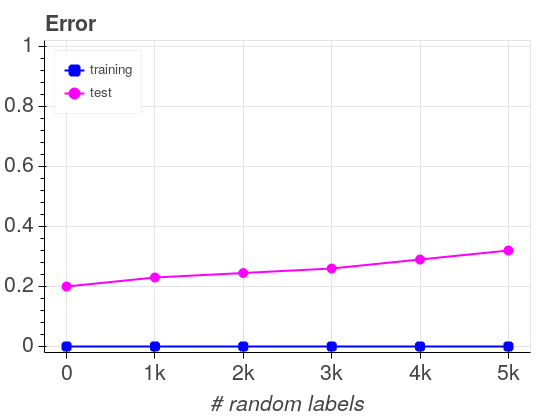
\includegraphics[width=0.24\linewidth]{vgg16/confusion/errors_01.png}
	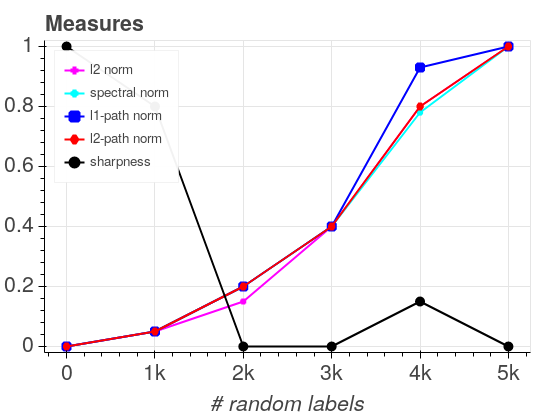
\includegraphics[width=0.24\linewidth]{vgg16/confusion/measures.png}
	\caption{The test and training error on the subset of CIFAR-10 and varying confusion set sizes (left) and the corresponding proposed capacity measures (right). Reproduced from \cite{neyshabur2017exploring}.}	
	\label{fig:confusion-paper}
\end{figure}
\begin{figure}
\centering
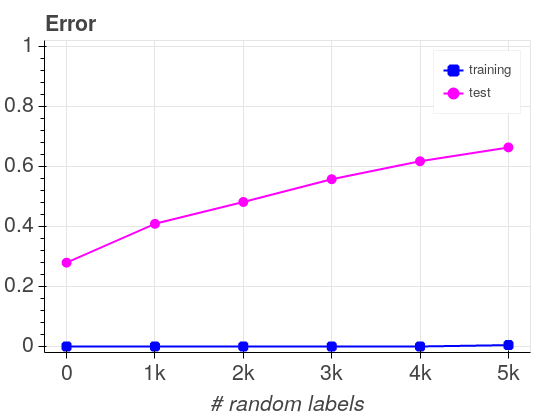
\includegraphics[width=0.24\linewidth]{vgg16/confusion/errors_own.png}
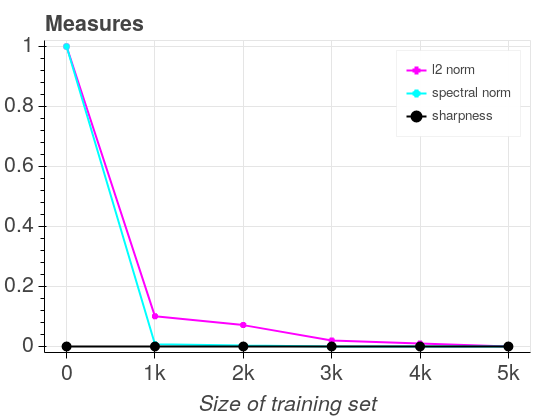
\includegraphics[width=0.24\linewidth]{vgg16/confusion/measures_own.png}
\caption{Our own results for the test and training error on the subset of CIFAR-10 and varying confusion set sizes (left) and the corresponding proposed capacity measures (right).}	
\label{fig:confusion-own}
\end{figure}
%
\subsubsection{Problems reproducing results}
We faced most of the problems already described in \ref{sec:problems-subset-sizes}. Especially the missing model and solving strategy details \ref{sec:problems-reproduction-training} as well as the calculation of the norms \ref{sec:problems-calculation-norms} prevented us from reproducing meaningful results. Nonetheless, the results are displayed in \freff{fig:confusion-own}.
%
\paragraph{Training to zero training loss not possible}
For the biggest confusion set size training to zero training loss was not possible. We tried different optimization strategies and hyper parameters but couldn't drive the model to zero training loss.
%
%
%
%
%%%%%%%%%%%%%%%%%%%%%%%%%%%%%%%%%%%%%%%%%%%%%%%%%%%%%%%%%%%%%%%%%%%%%%%%%%%%%%%%%%%%%%%%%%%%%%%%%%%%%%%%%%%%%%%%%%%%%%%%%%%%%%%%%%
%
%
%
\subsection{Implications of different hidden unit sizes}
Increasing the number of hidden units, thereby increasing the number of parameters, can
lead to a decrease in generalization error even when the training error does not decrease.
We would expect to see the complexity measure decrease as we increase the number of
hidden units. \cite{neyshabur2017exploring} 

%!TEX root=./report.tex
\section{Conclusion}
We saw that the norm-based capacity controls provide a good direction into understanding the empirical phenomena that correlate with the generalization ability of deep neural networks, but also that they alone are not sufficient to explain every phenomenon and further research is necessary. For sharpness, we have seen that it does not provide a valid capacity measure on its own and that it is not sufficient to ensure generalization. \ns{} provide some further investigation of expected sharpness in the PAC-Bayesian framework and how they can be combined to provide a capacity measure.

\newpage

%!TEX root=./report.tex
\newpage
\section{Appendix}
\begin{figure}[h!]
	\centering
	\includegraphics[width=0.49\linewidth]{cifar10}
	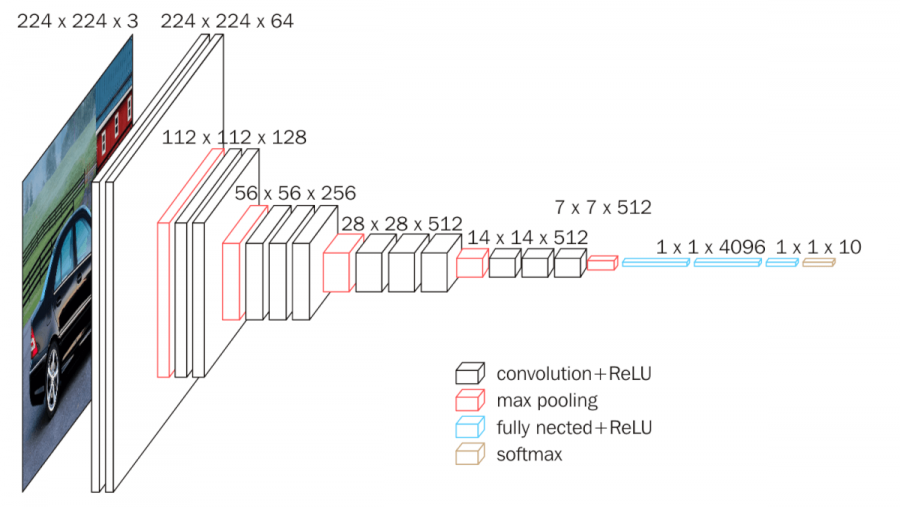
\includegraphics[width=0.49\linewidth]{vgg16}
	\caption{Left: A subset of the CIFAR-10 small image data set with ten classes. Right: The used implementation of the VGG-16 network with batch normalization. \cite{cifar10, vgg16}}	
	\label{fig:cifar-vgg}
\end{figure}

\begin{figure}[h!]
	\centering
	\includegraphics[width=0.45\linewidth]{mnist}
	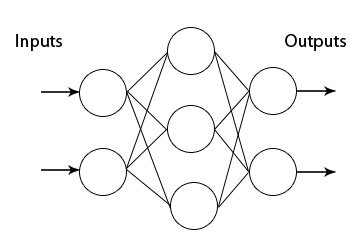
\includegraphics[width=0.45\linewidth]{two_layer_perceptron}
	\caption{Left: A subset of the MNIST handwritten digit data set. Right: An exemplary two layer perceptron with one input layer, one hidden layer of hidden unit size three and one output layer. \cite{mnist, two-layer-perceptron}}	
	\label{fig:mnist-two-layer}
\end{figure}

\begin{figure}[h!]
	\centering
	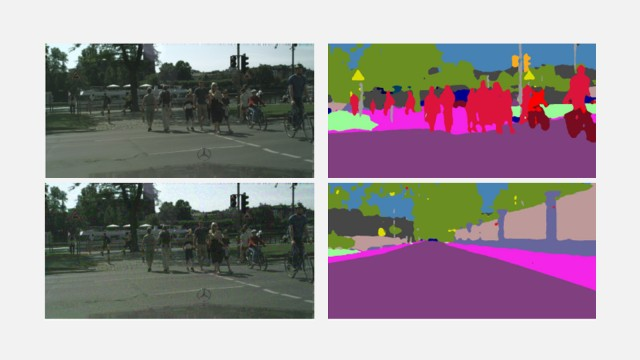
\includegraphics[width=0.8\linewidth]{bosch}
	\caption{Upper row: The original image (left) and the correct segmentation mask (right). Lower~row: The image with some additive adversarial perturbation barely visible to the human eye (left) and the corresponding wrong segmentation mask (right). \cite{metzen2017universal}}	
	\label{fig:adversarial-perturbations}
\end{figure}

\newpage

\nocite{*}

\bibliographystyle{plain}
\bibliography{egbib}



\end{document}
